
\section{Class System}
\subsection{Outline}

\begin{frame}
  \centering
  {\huge
    Week 1 -- Part 2: How this lecture is organized
  }
\end{frame}

\begin{frame}
  \frametitle{Outline}
  \begin{enumerate}
    \item Class Schedule
    \item Class Materials
    \item How to submit problems
    \item Grading
    \item Office Hours and Teacher Communication
    \item \alert{Special} Distance Learning in 2020
  \end{enumerate}
\end{frame}

\subsection{Class Schedule}
\begin{frame}{What you will do every week}
\end{frame}

\begin{frame}{Class Dates and Deadlines}
\end{frame}

\subsection{Class Materials}
\begin{frame}{Lecture Notes and Manaba}
\end{frame}
\begin{frame}{Online Judge Site}
\end{frame}
\begin{frame}{Course Language}
\end{frame}
\begin{frame}{Reference Books}
\end{frame}

\subsection{Problem Submission}
\begin{frame}{Submitting Assignments: Outline}
\end{frame}
\begin{frame}{What is OnlineJudge.org?}
\end{frame}
\begin{frame}{Submitting Problems to OnlineJudge.org}
\end{frame}
\begin{frame}{Attention: Java users}
\end{frame}
\begin{frame}{Reading the Judge Results}
\end{frame}
\begin{frame}{Submitting your code to Manaba}
\end{frame}

% \subsection{Tutorial}
% \begin{frame}
%   \frametitle{Tutorial: ``Relational Operator'' (1)}
%
%   All challenges are listed at the page:\\
%   {\smaller \url{http://conclave.cs.tsukuba.ac.jp/lecture/monitor.html}}
%
%   \bigskip
%
%   Let's click on "Relational Operator"
%
%   \begin{center}
%     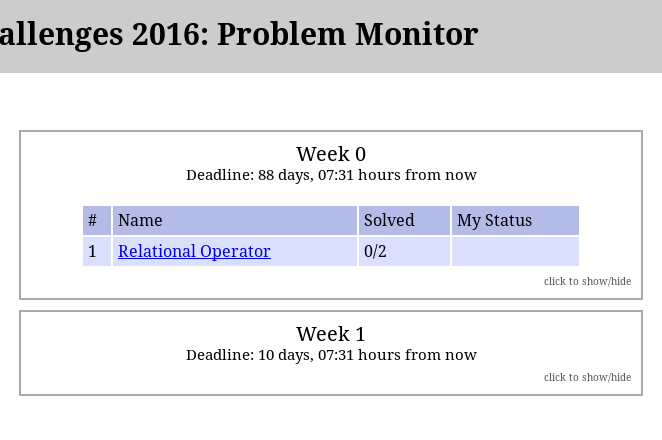
\includegraphics[width=.7\textwidth]{../img/monitorpage}
%   \end{center}
%
% \end{frame}
%
% \begin{frame}
%   \frametitle{Tutorial: ``Relational Operator'' (2)}
%
%   The link takes you to the UVA (University of Valladolid) homepage (\alert{Please use an ad blocker!}).
%
%   \bigskip
%
%   Here you can see the problem description, and the links to submit the problem.
%
%   \begin{center}
%     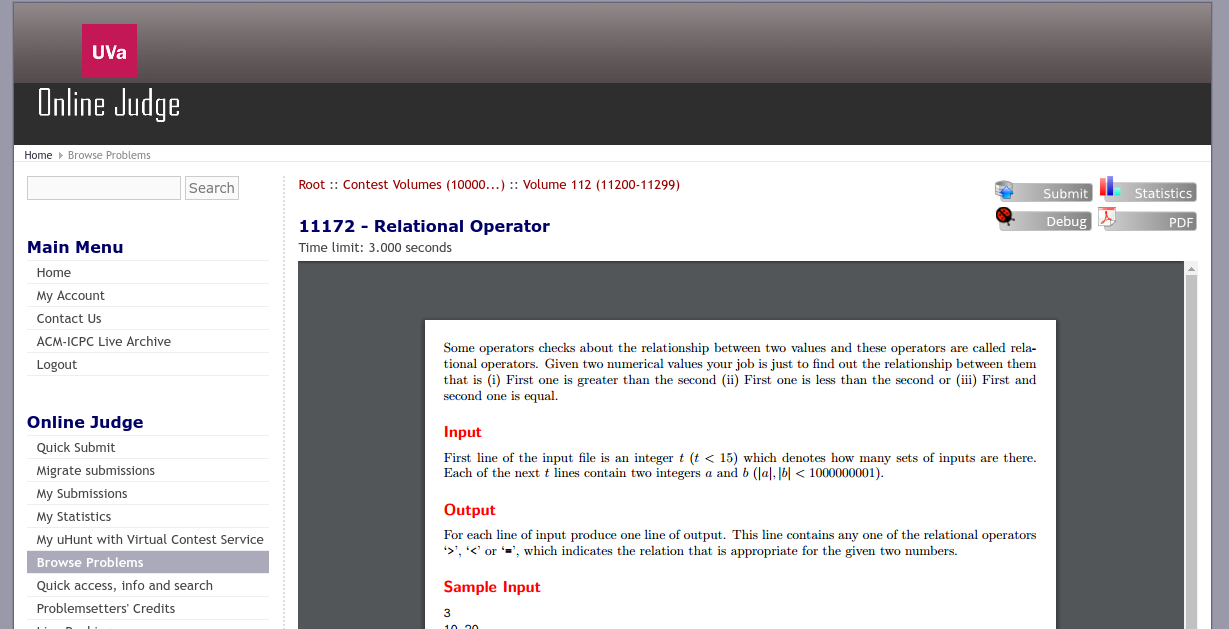
\includegraphics[width=.9\textwidth]{../img/relationaloperator}
%   \end{center}
% \end{frame}
%
% \begin{frame}
%   \frametitle{Tutorial: ``Relational Operator'' (3)}
%
%   \begin{block}{Description}
%     {\smaller \emph{
%     Some operators checks about the relationship between two values and these
%     operators are called relational operators. Given two numerical values \alert{your
%     job is} just to find out the relationship between them that is (i) First one
%     is greater than the second (ii) First one is less than the second or (iii)
%     First and second one is equal.}}
%   \end{block}
%
%   \begin{itemize}
%     \item Reading the description can be the hardest part!
%     \item For this challenge, you just need to:
%     \begin{itemize}
%       \item If the first number is bigger than the second; print ">"
%       \item If the first number is smaller than the second; print "<"
%       \item If both numbers are equal, print "="
%     \end{itemize}
%   \end{itemize}
%   Very easy!
% \end{frame}
%
%
% \begin{frame}
%   \frametitle{Tutorial: ``Relational Operator'' (4)}
%
%   \begin{block}{Input and Output}
%     {\smaller
%     \alert{Input}\\
%     First line of the input file is an integer $t (t < 15)$ which denotes how many sets of inputs are there.
%     Each of the next t lines contain two integers a and b (|a|, $|b| < 1000000001$).
%     \medskip
%
%     \alert{Output}\\
%     For each line of input produce one line of output. This line  contains any one of the relational operators
%     ''>'', ''<'' or ''='', which indicates the relation that is appropriate for the given two numbers.
%   }
%   \end{block}
%
%   \begin{itemize}
%     \item It is important to read the \alert{size} of the problem!
%     \item Pay attention to the \alert{shape} of the output!
%   \end{itemize}
%
% \end{frame}
%
% \begin{frame}
%   \frametitle{Tutorial: ``Relational Operator'' (5)}
%   \begin{block}{Examples}
%   \alert{Sample Input}\\
%   3\\
%   10 20\\
%   20 10\\
%   10 10\\
%   \alert{Sample Output}\\
%   <\\
%   >\\
%   =\\
%   \end{block}
%
%   \begin{itemize}
%     \item Use the samples to test/debug your program.
%     \item Use your own samples too!
%     \item Use the samples to \structure{understand} the challenge.
%   \end{itemize}
% \end{frame}
%
%
%
% \begin{frame}[fragile]
%   \frametitle{Solution: C++}
%
% \begin{block}{}
% {\smaller
% \begin{verbatim}
% // UVA 11172 - Relational Operator
% // Test if a is bigger, smaller or equal to b
%
% #include <iostream>
% using namespace std;
%
% int main()
% {
%     int n; long a, b;
%
%     cin >> n;
%     for (; n > 0; n--)
%     {
%         cin >> a >> b;
%         if (a > b) cout << ">\n";
%         if (a < b) cout << "<\n";
%         if (a == b) cout << "=\n";
%     }
% }
% \end{verbatim}}
% \end{block}
% \end{frame}
%
% \begin{frame}[fragile]
%   \frametitle{Solution: Python}
%   \begin{block}{}
% \begin{verbatim}
% n = int(input())
%
% while (n > 0):
%    line = input()
%    tokens = line.split()
%    a,b = int(tokens[0]),int(tokens[1])
%
%    if a > b: print(">")
%    if a < b: print("<")
%    if a == b: print("=")
%
%    n -= 1
% \end{verbatim}
%   \end{block}
%
% \end{frame}
%
% \begin{frame}[fragile]
%   \frametitle{Solution: Java}
%
%   {\tiny
%   \begin{block}{}
% \begin{verbatim}
% import java.io.*;
% class Main
% {
%    public static void main(String args[])
%    {
%       BufferedReader stdin = new BufferedReader(new InputStreamReader(System.in));
%       BufferedWriter stdout = new BufferedWriter(new OutputStreamWriter(System.out));
%       try {
%       String line;
%       line = stdin.readLine();
%       int n = Integer.parseInt(line);
%
%       for (int i = 0; i < n; i++)
%       {
%          line = stdin.readLine();
%          String[] tokens = line.split("\\s+");
%          long a = Integer.parseInt(tokens[0]);
%          long b = Integer.parseInt(tokens[1]);
%
%          if (a > b)
%             stdout.write(">\n");
%          if (a < b)
%             stdout.write("<\n");
%          if (a == b)
%             stdout.write("=\n");
%          stdout.flush();
%       }
%       stdout.close();
%       } catch (IOException ioe) { System.out.println("I/O Exception");}
%    }
% }
% \end{verbatim}
%   \end{block}
%   }
% \end{frame}
%
% \begin{frame}
%   \frametitle{Java Solution -- Keep in Mind}
%
%   \begin{itemize}
%   \item All code must be in the one file;
%
%     \medskip
%
%   \item The \structure{static main} method must be in \structure{Main} class.
%
%     \medskip
%
%   \item Do not use public classes. Even Main must be non public.
%
%     \medskip
%
%   \item Use Buffered I/O for faster input/output.
%   \end{itemize}
% \end{frame}
%
% \subsection{Submitting Your Program}
%
% \begin{frame}
%   \frametitle{Submitting the problem to UVA}
%   \begin{center}
%     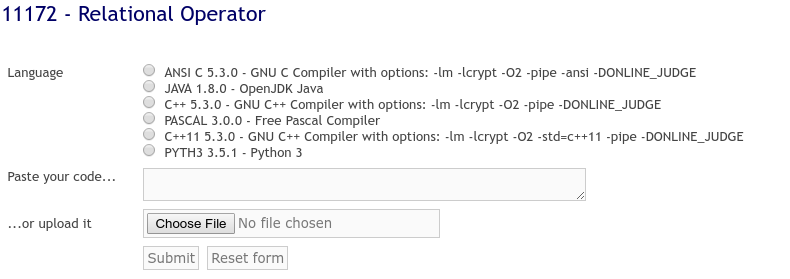
\includegraphics[width=1.1\textwidth]{../img/submitpage}
%   \end{center}
%
%   \begin{itemize}
%     \item After you complete the program, use the \structure{submit} button in the UVA page;
%     \item Choose your language and submit your code;
%     \item You can choose C, C++, Java or Python.
%   \end{itemize}
% \end{frame}
%
% \begin{frame}
%   \frametitle{Submitting the problem to UVA}
%
%     \begin{center}
%       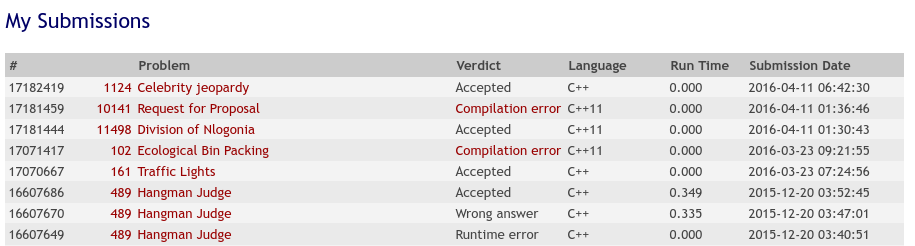
\includegraphics[width=1.1\textwidth]{../img/submissionpage}
%     \end{center}
%
%     \begin{itemize}
%       \item UVA has an \structure{Automated Judge}.
%       \item After 2~5 minutes, you should receive an e-mail with the result.
%       \item All your results can be seen at "My Submissions" Page.
%     \end{itemize}
% \end{frame}
%
% \begin{frame}
%   \frametitle{Submitting the problem to UVA}
%
%   These are the possible results:
%
%   \bigskip
%
%   \begin{itemize}
%   \item \structure{Accepted}: Your program is correct!
%     Congratulations!
%   \item \structure{Presentation Error}: Small mistake in number of spaces. Congratulations!
%
%     \bigskip
%
%   \item \alert{Wrong Answer}: Your program is incorrect. Time to debug.
%
%     \bigskip
%
%   \item \alert{Time Limit Exceeded}: Your program is too slow.
%
%   \item \alert{Memory limit exceeded}: Your program uses too much memory.
%
%     \bigskip
%   \item \alert{Runtime Error}: Your program crashed (segmentation fault!)
%
%     \bigskip
%   \end{itemize}
%
% \end{frame}
%
% \begin{frame}
%   \frametitle{Problem Monitor Page}
%
%
%   \begin{center}
%     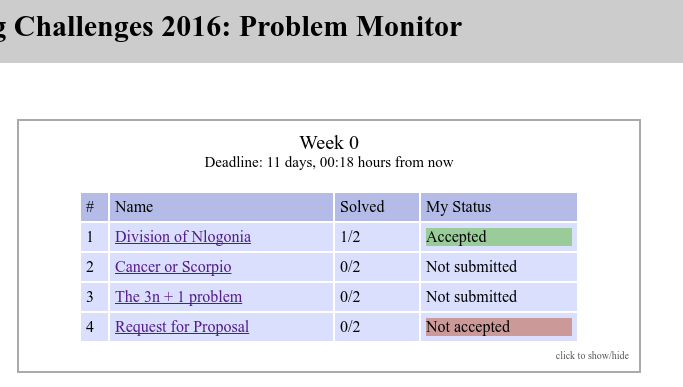
\includegraphics[width=1\textwidth]{../img/monitorpage2}
%   \end{center}
%
%   \begin{itemize}
%     \item All Problems and results;
%     \item All Deadlines;
%   \end{itemize}
%
% \end{frame}
%
% \subsection{Manaba Submission}
% \begin{frame}
%   \frametitle{Submitting the problem to MANABA}
%
%   {\small
%   After you finish the problems listed in the monitor, you need to
%   submit your source code and a comment file as a zip package to MANABA.}
%
%   \medskip
%
%   {\small
%   \begin{columns}
%     \column{0.3\textwidth}
%     \column{0.4\textwidth}
%     \begin{block}{s2015XXXXXX-weekYY.zip}
%       \begin{itemize}
%       \item problem1.cpp
%       \item problem2.cpp
%       \item problem5.cpp
%       \item kaisetsu.txt
%       \end{itemize}
%     \end{block}
%     \column{0.3\textwidth}
%   \end{columns}
%   }
%
%   \medskip
%
%   \begin{alertblock}{Attention}
%   Submission to the UVA judge without a submission to MANABA will not
%   be accepted!
%   \end{alertblock}
% \end{frame}



\subsection{Grading}
\begin{frame}{Grading Outline}
\end{frame}

\begin{frame}{Base Grade}
\end{frame}

\begin{frame}{Late Penalty}
\end{frame}

\begin{frame}{Best of Class Bonus}
\end{frame}

\begin{frame}{Plagiarism Warning}
\end{frame}

% \begin{frame}
%   \frametitle{Grading Algorithm}
%
%   Your Grade: {\bf Base Grade} \structure{+Bonus} \alert{-Penalty}
%
%   \begin{itemize}
%     \item {\bf Base Grade}:
%     \begin{itemize}
%       \item You solved 2/8 problem/week: "C"
%       \item You solved 3/8 problems/week: "B"
%       \item You solved 4/8 problems/week: "A"
%     \end{itemize}
%
%     \bigskip
%
%     \item \structure{+Bonus}
%     \begin{itemize}
%       \item 5\% of best student in each category.
%       \item Special collaboration to the class.
%     \end{itemize}
%
%     \bigskip
%     \item \alert{-Penalty}
%     \begin{itemize}
%       \item More than 25\% of homework submitted late.
%     \end{itemize}
%   \end{itemize}
%
%
% \end{frame}


% \begin{frame}
%   \frametitle{Evaluation and Grading (5) -- about plagiarism}
%
%   The assignments are \alert{individual}. Use your \structure{own
%     strength} to solve the programs.
%
%   \begin{exampleblock}{GOOD}
%     \begin{itemize}
%     \item Ask for ideas to your friends;
%     \item Ask for ideas in the MANABA forum;
%     \item Ask for help with a bug;
%     \end{itemize}
%   \end{exampleblock}
%
%   \begin{alertblock}{BAD}
%     \begin{itemize}
%     \item Copy a solution from the internet;
%     \item Copy a solution from your friends;
%     \item Give your code to a friend;
%     \end{itemize}
%   \end{alertblock}
%
%   Plagiarism will result in course failure, and possibly worse.
% \end{frame}


\subsection{Teacher Communication}
\begin{frame}{Teacher Communication}
\end{frame}

\begin{frame}{Using Manaba}
  % Alerts
  % Forums
\end{frame}

% \begin{frame}
%   \frametitle{Contact the professor}
%   \begin{itemize}
%   \item \structure{e-mail}: caranha@cs.tsukuba.ac.jp
%   \item \structure{website}: \url{http://conclave.cs.tsukuba.ac.jp}
%   %\item \structure{twitter}: @caranha
%
%     \bigskip
%
%   \item \structure{Room}: SB1012 -- Send an e-mail and we can talk!\\
%   \end{itemize}
%
%   \bigskip
%
%   Both English and Japanese are okay!
% \end{frame}


\subsection{Special 2020}
\begin{frame}{Special Considerations for 2020}
\end{frame}

\begin{frame}{Video Lectures and Lecture times}
\end{frame}

\begin{frame}{Submission Deadline and Programming Environment}
\end{frame}


%%%%%%%%%%%%%%%%%%%%%%%%%%%%%%%%%%%%%%%%%%%%%%
% \subsection{Course Outline}
% \begin{frame}
%   \frametitle{First Things First: Important Notices}
%
%   \begin{block}{Manaba Page}
%     All lecture notes and announcements for this course will be done
%     through MANABA. Access the url below:
%
%     \medskip
%
%     \url{https://manaba.tsukuba.ac.jp/ct/course_1149028}\\
%     Registration Code: 7255921
%   \end{block}
%   \begin{exampleblock}{Language}
%     \begin{itemize}
%       \item \structure{Lectures}: Japanese
%       \item \structure{Slides and materials}: English
%       \item \structure{Exercises}: English
%       \item \structure{Questions, Mails and Homework}: Any language
%     \end{itemize}
%   \end{exampleblock}
% \end{frame}


%%%%%%%%%%%%%%%%%%%%%%%%%%%%%%%%%%%%%%%%%%%%%%%%%%%%%
% \begin{frame}
%   \frametitle{Useful Links}
%   \begin{itemize}
%   \item
%     \href{https://manaba.tsukuba.ac.jp/ct/course_1149028}
%          {\structure{\underline{Manaba Page}}}: All the class material
%          will be here. Access Code is: 7255921
%
%     \medskip
%
%   \item \href{https://uva.onlinejudge.org/}{\structure{\underline{UVA Online Judge}}}:
%     Use this page to submit your problems. \alert{Make an account and list the username on MANABA}
%
%     \medskip
%
%   \item \href{https://conclave.cs.tsukuba.ac.jp/lecture/monitor.html}{\structure{\underline{Problem Monitor}}}:
%     Use this page to check deadlines and weekly problems.
%
%     \medskip
%
%   \item
%     \href{https://www.github.com/caranha/ProgrammingChallengesLectureNotes}{\structure{\underline{Github
%           Repository}}}:
%     Working directory for lecture notes. Send me PR, issues!
%
%     \medskip
%
%   \item
%     \href{https://www.udebug.com/}{\structure{\underline{uDebug}}}:
%     Web service that generates test inputs and test outputs for UVA
%     problems. Useful tool for this course.
%   \end{itemize}
% \end{frame}
%
%
% % Books
% % TODO: Add japanese books % Needs CJK package (or book images)
% \begin{frame}
%   \frametitle{Course Book}
%
%   \begin{itemize}
%   \item Competitive Programming, 3rd Edition
%     (\href{http://cpbook.net/}{http://cpbook.net})
%
%     \bigskip
%
%   \item For suggestions of books in Japanese, please check the Manaba materials!
%   \end{itemize}
% \end{frame}
%
% % udebug
% \begin{frame}
%   \frametitle{uDebug Tool}
%
%   uDebug generates outputs for many different debugs. It can help you check why your program is wrong.
%
%   \bigskip
%
%   \url{https://www.udebug.com/}
%
%   \bigskip
%
%   \begin{center}
%     
\includegraphics[width=0.7\textwidth]{../img/udebug}
%   \end{center}
% \end{frame}
